\documentclass{article}

\usepackage[english, russian]{babel}
\usepackage[letterpaper,top=2cm,bottom=2cm,left=3cm,right=3cm,marginparwidth=1.75cm]{geometry}

\usepackage{amsmath}
\usepackage{graphicx}
\usepackage{amsfonts}
\usepackage{amssymb}
\usepackage{amsthm}
\usepackage{mathtools}
\usepackage{graphicx}
\usepackage{epsfig}
\usepackage{caption}
\usepackage{float}
\usepackage[colorlinks=true, allcolors=blue]{hyperref}

\graphicspath{{images/}}

\newcommand{\bfv}[1]{\mathbf{#1}}
\newcommand{\dd}[1]{\dot{#1}}
\newcommand{\dvp}[3]{#1\,\times\,[\,#2\,\times\,#3\,]}
\newcommand{\dv}[1]{\nabla v(#1)}
\newcommand{\ddv}[1]{\mathrm{D}[v](#1)}
\newcommand{\dr}{\delta \bfv{r}}
\newcommand{\dn}{\delta \bfv{n}}
\newcommand{\om}[1]{\mathrm{o}(#1)}
\newcommand{\dprod}[2]{\langle #1, #2 \rangle}
\newcommand{\T}[1]{#1^\mathrm{T}}
\newcommand{\matr}[1]{\mathrm{#1}}
%\title{Your Paper}
%\author{You}

\begin{document}

\section{Постановка задачи}
Рассмотрим исходную систему бихарактеристик луча в переменных $\bfv{r}$ и $\bfv{n}$:
\begin{equation} \label{eq:1}
\begin{cases}
\dd{\bfv{r}} = v(\bfv{r})\,\bfv{n}\\
\dd{\bfv{n}} = \dvp{\bfv{n}}{\bfv{n}}{\dv{\bfv{r}}}\\
\end{cases}
\end{equation}
с начальными условиями $\bfv{r}|_{\tau=0} = \bfv{r}_0$ и $\bfv{n}|_{\tau=0} = \bfv{n}_0$\\\\
Из физических соображений $\bfv{n}$ --- единичная нормаль к волновому фронту $\Rightarrow \ \|\bfv{n}\| = 1$.\\\\
Воспользуемся тождеством Лагранжа для двойного векторного произведения $\dvp{\bfv{n}}{\bfv{n}}{\dv{\bfv{r}}}$:
\begin{equation} \label{eq:2}
    \dvp{\bfv{n}}{\bfv{n}}{\dv{\bfv{r}}} = \bfv{n}\,\dprod{\bfv{n}}{\dv{\bfv{r}}} - \dv{\bfv{r}}\,\dprod{\bfv{n}}{\bfv{n}} = \bfv{n}\,\dprod{\bfv{n}}{\dv{\bfv{r}}} - \dv{\bfv{r}}
\end{equation}\\
Подставляя \eqref{eq:2} в \eqref{eq:1}, получим:\\
\begin{equation} \label{eq:3}
\begin{cases}
\dd{\bfv{r}} = v(\bfv{r})\,\bfv{n}\\
\dd{\bfv{n}} =  \bfv{n}\,\dprod{\bfv{n}}{\dv{\bfv{r}}} - \dv{\bfv{r}}\\
\end{cases}
\end{equation}\\
Рассмотрим малое возмущение для $\bfv{r}$ и $\bfv{n}$:
\begin{align*}
\bfv{r_1} &= \bfv{r} + \dr   &   \bfv{n_1} &= \bfv{n} + \dr
\end{align*}
Будем считать, что в линейном приближении система \eqref{eq:3} верна для переменных $(\bfv{r_1}\,\bfv{n_1})$, то есть: 
\begin{equation} \label{eq:4}
\begin{cases}
\dd{\bfv{r_1}} = v(\bfv{r_1})\,\bfv{n_1} + \om{\|\dr\| + \|\dn\|}\\
\dd{\bfv{n_1}} = \bfv{n_1}\,\dprod{\bfv{n_1}}{\dv{\bfv{r_1}}} - \dv{\bfv{r_1}} + \om{\|\dr\| + \|\dn\|}\\
\end{cases}
\end{equation}\\
Разложим в ряд Тейлора функции $v(\bfv{r})$ и $\dv{\bfv{r}}$:
\begin{gather*} 
v(\bfv{r_1}) = v(\bfv{r}) + \dprod{\dv{\bfv{r}}}{\dr} + \om{\|\dr\|}\\ 
\dv{\bfv{r_1}} = \dv{\bfv{r}} + \ddv{\bfv{r}}\,\dr + \om{\|\dr\|}
\end{gather*}
Подставим полученные разложения в систему \eqref{eq:4}, воспользовавшись формулой Лагранжа для двойного векторного произведения: 
\begin{equation} \label{eq:5}
\begin{cases}
\dd{\bfv{r}} + \dd{\dr} = v(\bfv{r})\,\bfv{n} + \dprod{\dv{\bfv{r}}}{\dr}\,\bfv{n} + v(\bfv{r})\,\dn + \om{\|\dr\| + \|\dn\|}\\
\dd{\bfv{n}} + \dd{\dn} = \bfv{n}\,\dprod{\bfv{n}}{\dv{\bfv{r}}} - \dv{\bfv{r}} + \dn\,\dprod{\bfv{n}}{\dv{\bfv{r}}} + \bfv{n}\,\dprod{\dn}{\dv{\bfv{r}}} + \\ 
\qquad + \bfv{n}\,\dprod{\bfv{n}}{\ddv{\bfv{r}}\dr} - \ddv{\bfv{r}}\dr + \om{\|\dr\| + \|\dn\|}\\
\end{cases}
\end{equation}\\
Используя равенства системы \eqref{eq:1}, перепишем \eqref{eq:5} в следующем виде:
\begin{equation*}
\begin{cases}
\dd{\dr} = \dprod{\dv{\bfv{r}}}{\dr}\,\bfv{n} + v(\bfv{r})\,\dn + \om{\|\dr\| + \|\dn\|}\\
\dd{\dn} = \dn\,\dprod{\bfv{n}}{\dv{\bfv{r}}} + \bfv{n}\,\dprod{\dn}{\dv{\bfv{r}}} + \bfv{n}\,\dprod{\bfv{n}}{\ddv{\bfv{r}}\dr} - \ddv{\bfv{r}}\dr + \om{\|\dr\| + \|\dn\|}
\end{cases}
\end{equation*}
Что эквивалентно следующей записи:
\begin{equation} \label{eq:6}
\begin{cases}
\dd{\dr} = \bfv{n}\T{\dv{\bfv{r}}}\,\dr + v(\bfv{r})\,\dn + \om{\|\dr\| + \|\dn\|}\\
\dd{\dn} = \dprod{\bfv{n}}{\dv{\bfv{r}}}\,\dn + \bfv{n}\T{\dv{\bfv{r}}}\,\dn + \bfv{n}\T{\bfv{n}}\,\ddv{\bfv{r}}\,\dr - \ddv{\bfv{r}}\,\dr + \om{\|\dr\| + \|\dn\|}
\end{cases}
\end{equation}\\
В силу сферичности фронта положим $\dr = \matr{P}(\tau)\,\dn_0$ и $\dn = \matr{Q}(\tau)\,\dn_0$ и оставим только линейные $\delta$-члены. Сгруппируем по $\dn_0$, и в результате система \eqref{eq:6} примет вид:
\begin{equation} \label{eq:7}
\begin{cases}
\dd{\matr{P}} = \bfv{n}\T{\dv{\bfv{r}}}\,\matr{P} + v(\bfv{r})\,\matr{Q}\\
\dd{\matr{Q}} = (\bfv{n}\T{\bfv{n}} - \matr{I})\,\ddv{\bfv{r}}\,\matr{P} + (\bfv{n}\T{\dv{\bfv{r}}} + \dprod{\bfv{n}}{\dv{\bfv{r}}}\,\matr{I})\,\matr{Q} 
\end{cases}
\end{equation}
с начальными условиями: $\matr{P}|_{\tau=0} = \matr{\O}$ и $\matr{Q}|_{\tau=0} = \matr{I}$\\\\
\newpage
В матричном виде \eqref{eq:7}:
\begin{equation} \label{eq:8}
\begin{cases}
\dd{\matr{P}} = \matr{M}_{11}(\tau)\,\matr{P} + \matr{M}_{12}(\tau)\,\matr{Q}\\
\dd{\matr{Q}} = \matr{M}_{21}(\tau)\,\matr{P} + \matr{M}_{22}(\tau)\,\matr{Q} 
\end{cases}, \ \text{где}
\end{equation}\\
\begin{align*} 
&\matr{M}_{11}(\tau) = \bfv{n}(\tau)\T{\dv{\bfv{r}(\tau)}}&\matr{M}_{12}(\tau) = v(\bfv{r}(\tau))\,\matr{I}\\
&\matr{M}_{21}(\tau) = (\bfv{n}(\tau)\T{\bfv{n}(\tau)} - \matr{I})\,\ddv{\bfv{r}(\tau)}&\matr{M}_{22}(\tau) = \bfv{n}(\tau)\T{\dv{\bfv{r}(\tau)}} + \dprod{\bfv{n}(\tau)}{\dv{\bfv{r}(\tau)}}\,\matr{I}
\end{align*}

\subsection{Тестовые примеры}
Рассмотрим два наиболее простых поля скоростей для численной проверки рассмотренного ранее линейного приближения.

\subsubsection{Константное поле скоростей}
В первом примере положим $v(\bfv{r}) = a \ \forall \ r \in R$. Тогда легко видеть, что:
\begin{align*}
\dv{\bfv{r}} &= \T{(0,\,0,\,0)}  &   \ddv{\bfv{r}} &= \matr{\O}
\end{align*}
Следовательно, матрицы $\matr{M}_{11}$, $\matr{M}_{12}$, $\matr{M}_{21}$ и $\matr{M}_{22}$ системы \eqref{eq:8} примут следующий вид:
\begin{align*} 
&\matr{M}_{11}(\tau) = \matr{\O}&\matr{M}_{12}(\tau) = a\,\matr{I}\\
&\matr{M}_{21}(\tau) = \matr{\O}&\matr{M}_{22}(\tau) = \matr{\O}
\end{align*}
В результате получим следующую систему:
\begin{equation} \label{eq:9}
\begin{cases}
\dd{\matr{P}} = a\,\matr{Q}\\
\dd{\matr{Q}} = \matr{\O}\\
\matr{P}|_{\tau=0} = \matr{\O}; \ \matr{Q}|_{\tau=0} = \matr{I}
\end{cases}
\end{equation}
Ее решение легко находится:
\begin{equation} \label{eq:10}
\begin{cases}
\matr{P}(\tau) = a\tau\,\matr{I}\\
\matr{Q}(\tau) = \matr{I}
\end{cases}
\end{equation}
Положим для теста $a = 500$\,м/с, и рассмотрим численные значения следующих норм отклонений для различных моментов времени:\\
\begin{equation}
\|\bfv{r_1}(\tau) - (\bfv{r}(\tau) + \matr{P}(\tau)\,\dr)\|^2, \ \text{где $\bfv{r}_1$ -- решение \eqref{eq:4}, $\bfv{r}$ -- решение \eqref{eq:1}}
\end{equation}
\begin{figure}[H] 
\centering
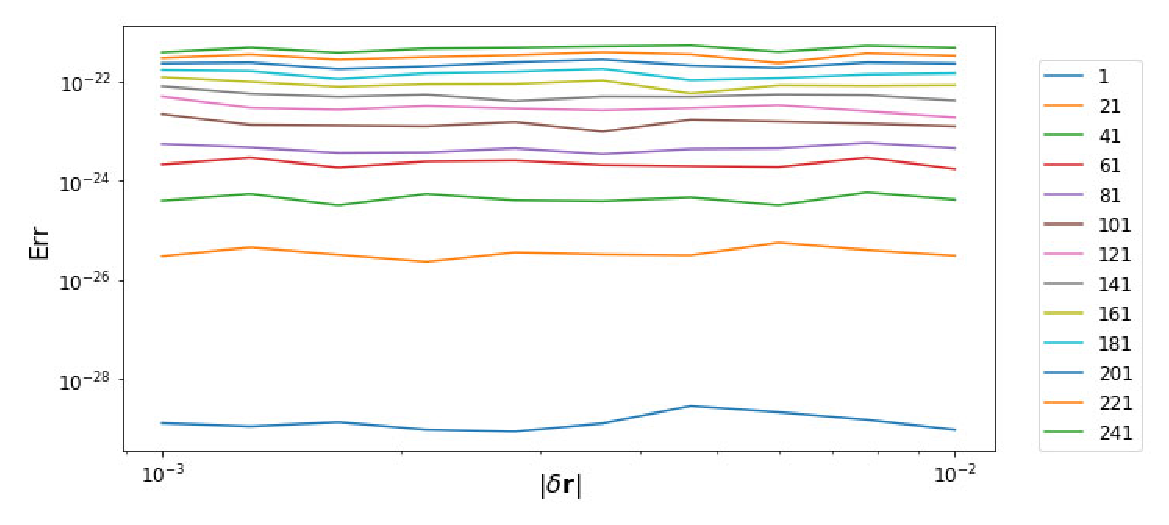
\includegraphics[width=1.0\linewidth]{Error_level_lines_const.eps}
\caption{Верхние огибающие для нормы ошибки для различных норм $\dr$ в заданные моменты времени $\tau$.}
\label{fig:1}
\end{figure}
Из рис. \ref{fig:1} легко видеть, что норма ошибки на несколько порядков меньше отклонения.

\subsubsection{Линейное поле скоростей}
Во втором примере положим $v(\bfv{r}) = a + b\,\bfv{r}_z$. Тогда:
\begin{align*}
\dv{\bfv{r}} &= \T{(0,\,0,\,b)}  &   \ddv{\bfv{r}} &= \matr{\O}
\end{align*}
Следовательно, матрицы $\matr{M}_{11}$, $\matr{M}_{12}$, $\matr{M}_{21}$ и $\matr{M}_{22}$ системы \eqref{eq:8} примут следующий вид:
\begin{align*} 
&\matr{M}_{11}(\tau) = \begin{bmatrix}
0 & 0 & b\,n_x\\
0 & 0 & b\,n_y\\
0 & 0 & b\,n_z
\end{bmatrix}&\matr{M}_{12}(\tau) = \begin{bmatrix}
a + b\,r_x & 0 & 0\\
0 & a + b\,r_y & 0\\
0 & 0 & a + b\,r_z
\end{bmatrix}\\\\
&\matr{M}_{21}(\tau) = \begin{bmatrix}
0 & 0 & 0\\
0 & 0 & 0\\
0 & 0 & 0
\end{bmatrix}&\matr{M}_{22}(\tau) = \begin{bmatrix}
b\,n_z & 0 & b\,n_x\\
0 & b\,n_z & b\,n_y\\
0 & 0 & 2\,b\,n_z
\end{bmatrix}
\end{align*}
В результате получим следующую систему:
\begin{equation} \label{eq:11}
\begin{cases}
\dd{\matr{P}} = \matr{M}_{11}(\tau)\,\matr{P} + \matr{M}_{12}(\tau)\,\matr{Q}\\
\dd{\matr{Q}} = \matr{M}_{22}(\tau)\,\matr{Q}\\
\matr{P}|_{\tau=0} = \matr{\O}; \ \matr{Q}|_{\tau=0} = \matr{I}
\end{cases}
\end{equation}
Легко видеть, что решение первого уравнения зависит от решения второго, однако решение второго не зависит от первого. Следовательно, система распадается на две системы из трех дифференциальных уравнений (в силу того, что матрицы $\matr{M}_{12}$ и $\matr{M}_{22}$ полного ранга), решаемых последовательно.\\
\begin{align*}
\begin{cases}
\dd{\matr{Q}} = \matr{M}_{22}(\tau)\,\matr{Q}\\
\matr{Q}|_{\tau=0} = \matr{I}
\end{cases}   
\quad & \quad   
\begin{cases}
\dd{\matr{P}} = \matr{M}_{11}(\tau)\,\matr{P} + \matr{M}_{12}(\tau)\,\matr{Q}\\
\matr{P}|_{\tau=0} = \matr{0}
\end{cases} 
\end{align*}\\
Положим для теста $a = 500$\,м/с, $b = -10$\,$\text{с}^{-1}$ и рассмотрим численные значения следующих норм отклонений для различных моментов времени:\\
\begin{equation}
\|\bfv{r_1}(\tau) - (\bfv{r}(\tau) + \matr{P}(\tau)\,\dr)\|^2, \ \text{где $\bfv{r}_1$ -- решение \eqref{eq:4}, $\bfv{r}$ -- решение \eqref{eq:1}}
\end{equation}
\begin{figure}[H] 
\centering
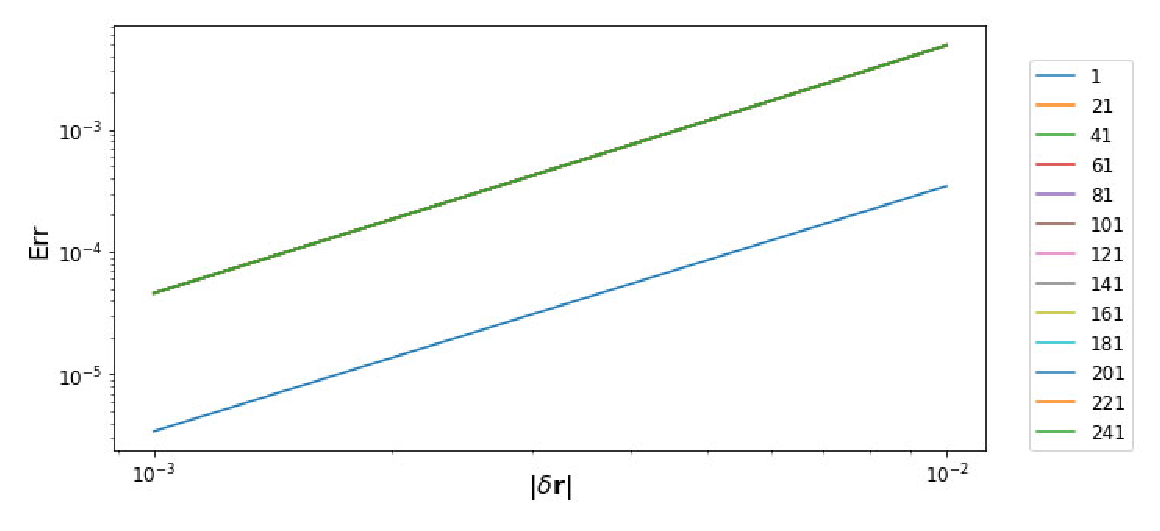
\includegraphics[width=1.0\linewidth]{Error_level_lines_lin.eps}
\caption{Верхние огибающие для нормы ошибки для различных норм $\dr$ в заданные моменты времени $\tau$.}
\label{fig:2}
\end{figure}
Из рис. \ref{fig:2} легко видеть, что норма ошибки имеет порядок отклонения. Также можно видеть, что начиная с $\tau = 0.2$\,с норма ошибки стабилизируется.
\end{document}
